% -*- TeX-master: "all_the_notes.tex" -*-

\section{Qubit-Resonator               System
  \cite{Blais_2004}}

\begin{framed}\noindent
  Please  see \autoref{sec:transmission-line}
  for a derivation formulas for the resonator
  itself.
\end{framed}

\begin{enumerate}
\item The  two-level qubit with  a separation
  between the energy  levels $ \Delta E  $ has the
  Hamiltonian

\begin{equation}
  \mathcal{H}_{a}= -\frac{\Delta E}{2}\sigma_z.
  \label{qrA}
\end{equation}

\item This qubit is placed in close proximi y
  with a resonator, which, as we have seen in
  the  previous   chapter,  has   a  harmonic
  oscillator-like Hamiltonian

\begin{equation}
  \mathcal{H}_{r}={\hbar\omega}\bigg(\red{\hat{N}}+\frac{1}{2}\bigg)\qquad \qquad a^{\dagger}\ket{N}=\sqrt{N+1}\ket{N+1}; \qquad a\ket{N}=\sqrt{N}\ket{N=1}.
  \label{qrR}
\end{equation}

\noindent where for simplicity we neglect the
constant energy term.

\item The  general state  of a  system, where
  the  qubit  is  in  state $  n  $  and  the
  resonator  in state  $  N $  (i.e.   $ N  $
  photons) will be

\begin{equation}
  \ket{n,N}.
\end{equation}

\noindent Qualitatively speaking, the way the
qubit interacts with the  resonator in one of
the two ways

\begin{itemize}
\item Qubit absorbs  a photon and transitions
  to        the         excited        state:
  $ \blue{\ket{0,N+1} \rightarrow \ket{1,N}} $;
\item  Qubit  relaxes  to  ground  state  and
  releases  a  photon   into  the  resonator:
  $ \red{\ket{1,N} \rightarrow \ket{0,N+1}} $.
\end{itemize}

This  can be  expressed  via the  interaction
Hamiltonian

\begin{equation}
  \mathcal{H}_{\text{int}}=\blue{a\sigma^+}+\red{a^{\dagger}\sigma^-}.
  \label{qrInt}
\end{equation}
\end{enumerate}
\begin{framed}\noindent
  \LARGE
  \[        \mathcal{H}       =\blue{-\frac{\Delta
        E}{2}\sigma_z}+\blue{{\hbar\omega_r}a^\dagger
      a}               +               \red{\hbar
      g_0\bigg({a\sigma^+}+{a^{\dagger}\sigma^-}\bigg)},
  \]
\end{framed}

\begin{figure}[h]
  \centering
  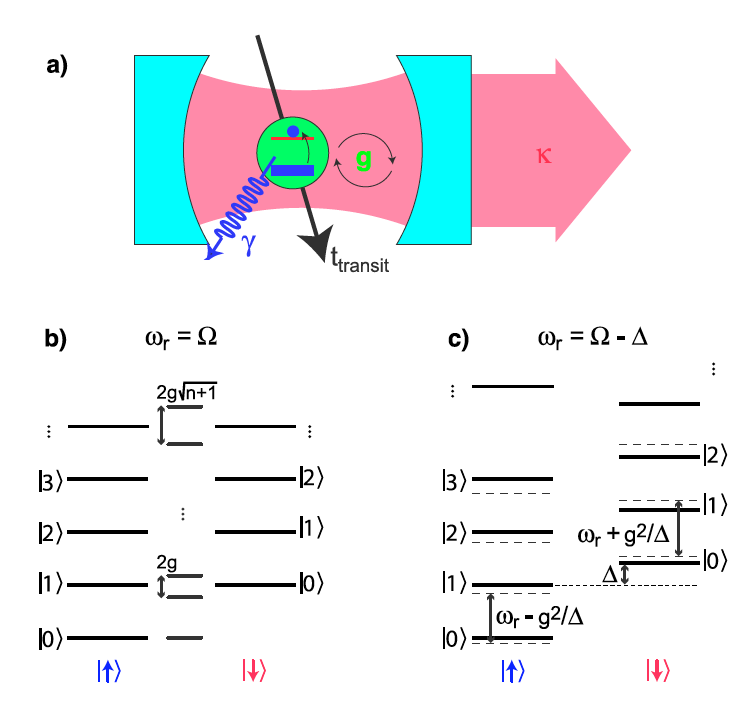
\includegraphics[height=8cm]{cavityPic1}
  \caption{Interaction  between  states  with
    same energy creates the superposed states
    in the middle. \label{qb_res_ladder}}
\end{figure}

\noindent  This gives  rise to  energy levels
depicted in  Fig.\ref{qb_res_ladder} which we
write  out  in  terms of  the  basis  states,
recalling                                that
$  \sigma_z=\iketbra{e}{e}-  \iketbra{g}{g}$,
$\sigma^+=\iketbra{e}{g}$,
$\sigma^-=\iketbra{g}{e}$,
$    a   =    \sqrt{N+1}\iketbra{N}{N+1}   $,
$ a^\dagger = \sqrt{N+1}\iketbra{N+1}{N} $:

\begin{equation}
  \begin{aligned}
    \mathcal{H} & = \blue{\bigg[\frac{\Delta E}{2}\big(\iketbra{e}{e}-\iketbra{g}{g}\big)\bigg]\otimes\mathbb{I}_{N}} + \blue{\mathbb{I}_{n}\otimes\bigg[\hbar\omega_r\sum_{N}N\iketbra{N}{N}\bigg]} +\\
    &\ +  \red{\hbar g_0\bigg[\iketbra{e}{g}\sqrt{N+1}\sum_{N}\iketbra{N}{N+1}+\iketbra{g}{e}\sum_{N}\sqrt{N+1}\iketbra{N+1}{N}\bigg]}\\
    & = \sum_{N}\quad\blue{\bigg(\hbar N\omega_r-\frac{\Delta E}{2}\bigg)\iketbra{g,N}{g,N}+\bigg(\hbar N\omega_r+\frac{\Delta E}{2}\bigg)\iketbra{e,N}{e,N} \leftarrow \text{ diagonal }}\\
    &\ +  \red{\hbar g_0\sqrt{N+1}\bigg[\iketbra{e,N}{g,N+1}+\iketbra{g,N+1}{e,N}\bigg] \leftarrow \text{ cross terms }}\\
  \end{aligned}
\end{equation}

\noindent and in matrix form

\begin{equation}\label{eqn:qubitCavityHamil}
  \mathcal{H} = \kbordermatrix{
    & \ket{g,N} & \ket{e,N} & \ket{g,N+1} & \ket{e,N+1} \\
    \bra{g,N} &\blue{\hbar N\omega_r-\frac{\Delta E}{2}} & 0 & 0 & 0\\
    \bra{e,N} & 0 & \blue{\hbar N\omega_r+\frac{\Delta E}{2}} & \red{\hbar g_0
      \sqrt{N+1}} & 0\\
    \bra{g,N+1} & 0 & \red{\hbar g_0\sqrt{N+1}} & \blue{\hbar (N+1)\omega_r-\frac{\Delta E}{2}} & 0\\
    \bra{e,N+1} & 0 & 0 & 0 & \blue{\hbar (N+1)\omega_r+\frac{\Delta E}{2}}.\\
  }
\end{equation}

\subsection{General solutions}
\begin{enumerate}
\item For  the ground state, we  take the top
  row, which will have the lowest energy
  \[
    \iket{g,0}     =    \begin{pmatrix}     1
      \\0\\\vdots
    \end{pmatrix}\text{ with energy }
    -\frac{\Delta E}{2}.
  \]

\item Then diagonalising  an arbitrary middle
  matrix    (N    value    incremented    for
  convenience)

  \begin{equation}\begin{aligned}
      \mathcal{H}_{\text{middle}}
      & = \kbordermatrix{&\ket{e,N} & \ket{g,N+1}\\
        \bra{e,N} & \blue{\hbar\omega_r(N+\frac{1}{2}) + \hbar\Delta} & \red{\hbar g_0\sqrt{N+1}}\\
        \bra{g,N+1} & \red{\hbar g_0\sqrt{N+1}} & \blue{\hbar\omega_r(N+\frac{1}{2}) - \hbar\Delta}}\\
      &= \blue{\hbar\omega_r(N+\frac{1}{2})\mathbb{I} +\frac{ \hbar\Delta}{2}\sigma_z} + \red{\hbar g_0\sqrt{N+1}\sigma_x}\\
      & = \blue{\hbar\omega_r(N+\frac{1}{2})\mathbb{I}} + \frac{1}{2}\sqrt{(\hbar\Delta)^2 + 4\hbar^2g_0^2(N+1)} \bigg(\cos(\theta)\sigma_z + \sin(\theta)\sigma_x\bigg)\\
      & = \hbar\omega_r(N+\frac{1}{2})\mathbb{I} + E_{\text{coupled}}(\cos(\theta)\sigma_z + \sin(\theta)\sigma_x)\\
      &  \text{where   }  E_\text{coupled}  =
      \frac{\hbar}{2}\sqrt{\Delta^2             +
        4g_0^2(N+1)};\qquad     \tan(\theta)     =
      \frac{g_0\sqrt{N+1}}{\Delta/2}.
    \end{aligned}
  \end{equation}

  \begin{framed}\noindent
    \paragraph{Rotated frame}


    \[             \mathcal{H'}             =
      \hbar\omega_r(N+\frac{1}{2})\mathbb{I}
      +    \frac{E_\text{coupled}}{2}\sigma_z
      =                       \begin{pmatrix}
        \hbar\omega_r(N+\frac{1}{2})        +
        \frac{E_\text{coupled}}{2}   &  0\\0&
        \hbar\omega_r(N+\frac{1}{2})        -
        \frac{E_\text{coupled}}{2}
      \end{pmatrix}
    \]
    \begin{itemize}
    \item         \textbf{Eigenstates}:\hfill
      \iket{\tilde{0}}, \iket{\tilde{1}};
    \item    \textbf{Eigenenergies}:   \hfill
      $    \hbar\omega_r(N+\frac{1}{2})   \pm
      \frac{E_\text{coupled}}{2} $.
    \end{itemize}
  \end{framed}

\item    By    applying   a    rotation    of
  $ \frac{\theta}{2} $ about the y-axis

  \[
    U =  \exp\big[i\frac{\theta}{2}\sigma_y\big] =
    \cos(\frac{\theta}{2})\mathbb{I}             +
    i\sin(\frac{\theta}{2})\sigma_y,
  \]

  \noindent we will end up with

  \begin{framed}\noindent
    \paragraph{Raw frame}


    \begin{itemize}
    \item \textbf{Eigenstates:}
      \[
        \begin{aligned}
          \iket{+,N} & = U^{\dagger}\ket{\tilde{1}}
          =
          \bigg(\cos(\frac{\theta}{2})\mathbb{I}-i\sin(\frac{\theta}{2})\sigma_y\bigg)
          \begin{pmatrix}1\\0 \end{pmatrix} =
          \begin{pmatrix} \cos(\frac{\theta}{2})\\\sin(\frac{\theta}{2})\end{pmatrix} \\
          \iket{-,N} & = U^{\dagger}\ket{\tilde{0}}
          =                   \begin{pmatrix}
            -\sin(\frac{\theta}{2})\\\cos(\frac{\theta}{2})
          \end{pmatrix} \equiv -\sin(\frac{\theta}{2})\iket{e,N} + \cos(\frac{\theta}{2})\iket{g,N+1}\\
        \end{aligned}
      \]
    \item    \textbf{Eigenenergies:}   \hfill
      $        \text{Energies}_{\pm}        =
      \hbar\omega_r(N+\frac{1}{2})        \pm
      \frac{E_\text{coupled}}{2} $
    \end{itemize}
  \end{framed}

\end{enumerate}

\begin{figure}[h]
  \centering
  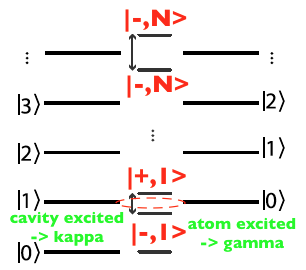
\includegraphics[height=5cm]{cavityPic2}
\end{figure}

\subsection{Resontant case}
\label{sec:resontant-case}



\noindent  The  eigenstate  spectrum  of  the
\iket{\pm,N} states is  ladder-like (down the
middle).   For   a  single  photon,   and  on
resonance ($  \Delta =  0 $) the  entangled states
are

 \[
   \iket{\pm,1}   =    \frac{\iket{e,0}   \pm
     \iket{g,1}}{\sqrt{2}}   \quad  \text{   with
     energies  } \hbar\omega_r(N+\frac{1}{2})
   \pm \hbar g_0\sqrt{N+1},
 \]

 \noindent   will  flip   flop  between   the
 original  levels   with  a   Rabi  frequency
 $ 2g_0/2\pi  $. As  the atom is  excited for
 exactly half of the state, with a decay rate
 $ \gamma  $ , and  the cavity is excited  for the
 other half  of the state, with  a decay rate
 $   \kappa    $   the    net   decay    rate   is
 $ \frac{\gamma+\kappa}{2}  $ and  to observe
 Rabi   oscillations  between   the  original
 states

 \[
   2g        >        \frac{\kappa+\gamma}{2}
   \qquad\qquad\text{\red{to     see     Rabi
       oscillation     before    decay     ==
       \textbf{strong coupling}}}
 \]

 \begin{framed}\noindent
   \begin{itemize}
   \item  If a  cavity is  resonant with  the
     atom,  then   the  atom  can   emit  and
     reabsorb       photons       coherently.
     Alternatively,  if   the  atom   is  far
     detuned  from  any   cavity  mode,  it’s
     eigenstates   are    very   nearly   the
     eigenstates of the system;
   \item The  rate at  which an  atomic level
     decays   is  proportional   (by  Fermi’s
     golden rule) to the density of states of
     the local electromagnetic  field at that
     atomic frequency;
   \item But  the mode  quantization enforced
     by  a cavity  redefines  the density  of
     states available to the atom, increasing
     it   in  the   case   of  resonance   or
     diminishing  it  in   the  case  of  far
     detuning.  By  this channel,  the cavity
     can  enhance or  reduce the  spontaneous
     emission  rate of  an atom  [20, 21]  in
     what is known as the Purcell effect.
   \end{itemize}
 \end{framed}

 \subsection{Non-resonant
   case}\label{sec:stark-shift}

 \begin{framed}\noindent
   In   the   case    that   large   detuning
   $\Delta >> g$ is applied (detuning is much
   greater than the coupling) we expand
   \begin{equation}
     \iket{\pm,1}      =     -\sin(\frac{\theta}{2})\iket{e,0}     +
     \cos(\frac{\theta}{2})\iket{g,1} \qquad \tan(\theta)     =
     \frac{g_0\sqrt{N+1}}{\Delta/2}.
   \end{equation}
   \noindent
 \end{framed}

 \begin{equation}
   \iket{-,1} \approx \frac{-g}{\Delta}\iket{e,0} + \iket{g,1}
 \end{equation}

 \begin{itemize}
 \item Atom decays at a rate $\frac{-g}{\Delta}$;
 \item Cavity decays at a rate 1;
 \item $\Gamma = (g/\Delta)^2\gamma+\kappa$
 \end{itemize}

 and
 \begin{equation}
   \iket{+,1} \approx  \iket{g,0}  +
   \frac{g}{\Delta}\iket{e,1}
 \end{equation}

 \begin{itemize}
 \item Atom decays at rate 1;
 \item Cavity decays at rate $\frac{-g}{\Delta}$;
 \item $\Gamma = \gamma+ (g/\Delta)^2\kappa$.
 \end{itemize}

 \noindent    If   we    apply   a    unitary
 transformation
 ($U  = \exp  \left( \frac{g}{\Delta}(a\sigma^+  +
   a^{\dagger}\delta^{-} \right)$):

 \begin{equation}\label{eq:resonator-stark-shift}
   \begin{aligned}
     U\mathcal{H}U^{\dagger} & \approx \hbar\omega_ra^{\dag}a + \left[\frac{\hbar\Omega}{2} + \blue{\frac{g^{2}}{\Delta}\left( a^{\dagger}a + \frac{1}{2} \right)} \right]\sigma_z \\
     &    =     \hbar    \left[     \omega_r    +
       \green{\frac{g^2}{\Delta}\sigma_z}
     \right]a^{\dagger}  a  +  \frac{\hbar}{2}\big[\Omega  +
     \frac{g^2}{\Delta}\big]\sigma_z
   \end{aligned}
 \end{equation}

 \noindent which we can interpret as

 \begin{framed}\noindent
   \begin{itemize}
   \item  \blue{\textbf{Stark/Lambda  shift}:
       photon-number-dependent  shift of  the
       atom's            energy            by
       $\frac{g^{2}}{\Delta}\left(     a^{\dagger}a    +
         \frac{1}{2} \right)$};
   \item    \green{\textbf{Dispersive   shift
         (cavity  energy shifts  by $\chi$):}
       The   atom    ``pulls''   the   cavity
       frequency by  $ \chi  = \pm  g^2/\Delta $
       depending on the atomic state} (we can
     neglect the  constant offset as  it will
     not affect transition energies.
   \end{itemize}

   \noindent  Because of  the Purcell  effect
   (cavity  limits density  of state  that an
   excited qubit  can decay  into) suppresses
   the   local  electromagnetic   density  of
   states  at  the detuned  qubit  frequency,
   thus inhibiting excited state decay.
 \end{framed}

 \noindent An  example of this effect  can be
 found  in  the  following  paper  about  SAW
 \cite{Manenti_2017}

\begin{figure}[h]
  \centering
  \inkfig{15cm}{ac_stark_effect_dispersive_shift}
  \caption{\small  When there  is 0  detuning
    (right,  $\hbar\omega_{r}=\Delta E$)  the
    dressed states create  a degeneracy which
    is lifted by the  coupling. When there is
    a  sizeable   detuning  $\Delta$  (left),
    there will  be no degeneracy.   Instead -
    per    \autoref{eq:resonator-stark-shift}
    the  energy  of  the  atom  shifts  by  a
    constant factor (not interesting) whereas
    the  resonator  ladder energy  separation
    changes                                by
    \green{$\pm\frac{g^{2}}{\Delta}$} depending on
    state                                  of
    atom. \label{fig:ac_stark_effect_dispersive_shift}}
\end{figure}

\newpage\subsection{Stark shift measurements}
\label{sec:stark-shift-meas}

Let  us  use  the  dispersive  shift  of  the
resonator frequency,  dependent on  the state
of the qubit as in \autoref{fig:stark-shift}.
Measurements can be done at either:
\begin{itemize}
\item $\omega_r'  \pm \chi $: amplitude  for the
  two state will be different;
\item $\omega_r'$:  phase for the  two states
  will be different (shifted by $\pi$).
\end{itemize}

\begin{figure}[h]
  \centering
  \includegraphics[height=5cm]{cqed/stark-shift}
  \caption{\small    There    will    be    2
    transmission  profiles, depending  on the
    state of the qubit. Transmission (dotted)
    vs phase (solid)\label{fig:stark-shift}}
\end{figure}

\noindent

\subsection{Resonant case = Dressed States}
\label{sec:resonant-case}

{\LARGE
  \[\hbar\omega_r \equiv \Delta E\]}
\begin{equation}
  \mathcal{H} = \kbordermatrix{
    & \ket{0,N-1} & \ket{1,N-1} & \ket{0,N} & \ket{1,N} \\
    \bra{0,N-1} &\blue{\Delta E\big(N-\frac{3}{2}\big)} & 0 & 0 & 0\\
    \bra{1,N-1} & 0 & \blue{\Delta E\big(N-\frac{1}{2}\big)} & \red{\hbar g_0\sqrt{N}} & 0\\
    \bra{0,N} & 0 & \red{\hbar g_0\sqrt{N}} & \blue{\Delta E\big(N-\frac{1}{2}\big)} & 0\\
    \bra{1,N} & 0 & 0 & 0 & \blue{\Delta E\big(N+\frac{1}{2}\big)}\\
  },
\end{equation}

\noindent  and a  degeneracy appears  between
the     two    middle     states    as     in
Fig.\ref{qrLevel}.   The middle  part of  the
Hamiltonian is treated as a two levels system

\begin{equation}
  \mathcal{H}_{\text{middle}} = \begin{pmatrix}
    \blue{\Delta E\big(N-\frac{1}{2}\big)} & \red{\hbar g_0\sqrt{N}}\\
    \red{\hbar g_0\sqrt{N}} & \blue{\Delta E\big(N-\frac{1}{2}\big)}
  \end{pmatrix}\qquad\Rightarrow\qquad\kbordermatrix{
    &\ket{1,N-1}&\ket{0,N}\\
    \bra{1,N-1}& 0 & \red{\hbar g_0\sqrt{N}}\\
    \bra{0,N}& \red{\hbar g_0\sqrt{N}} & 0},
\end{equation}

\noindent which can  be diagonalised with two
states     separated     by     an     energy
$   g_0\sqrt{N}    $,   also    depicted   in
Fig.\ref{qrLevel}.  The  degeneracy is lifted
for every single state,  and these states are
known as dressed.

\begin{equation}
  \ket{\Psi} = \frac{\ket{0,N}\pm\ket{1,N-1}}{\sqrt{2}} \qquad E = \pm{g_0\sqrt{N}}.
\end{equation}

\begin{figure}
  \centering
  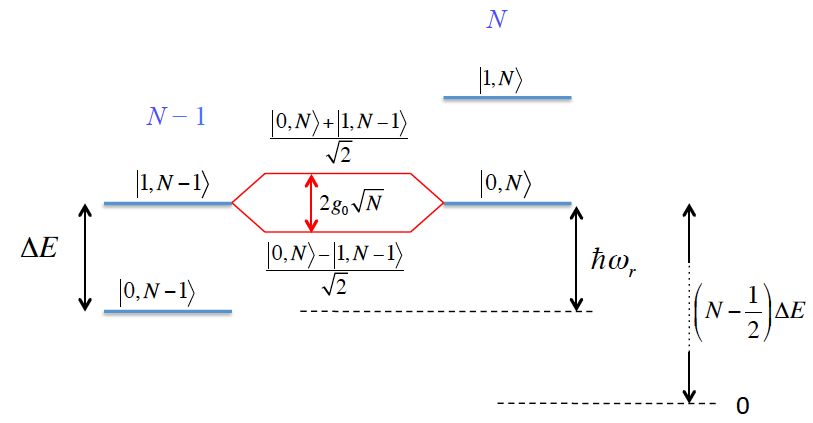
\includegraphics[height=6cm]{qrLevel}
  \caption{Degeneracy    between    different
    photon states \label{qrLevel}.  Note that
    relative    to     zero    energy    (for
    $   \ket{0,0}  $)   one  is   shifted  by
    $                  N\hbar\omega_r-\frac{\Delta
      E}{2}=\bigg(N-\frac{1}{2}\bigg)\Delta E $}
\end{figure}

Fig.\ref{qrDresssed}    is   intepreted    as
follows:

\begin{itemize}
\item  We have  a  qubit, that  is either  in
  state  \iket{0} or  \iket{1}, whose  energy
  spectrum is  shown by the green  lines.  By
  controlling some  bias e.g.   gate voltage,
  we    choose    the    energy    difference
  $ \Delta E $ between the two levels.
\item  We  apply a  \textbf{fixed}  resonator
  drive at  $ \hbar\omega_r $.  This  makes a
  copy of the  original qubit states, shifted
  by $  \hbar\omega_r $.   This configuration
  corresponds to the \blue{blue} terms in the
  above equations.
\item  At the  degeneracy point  for the  new
  qubit-resonator system,  degeneracy will be
  lifted  by the  qubit-resonator interaction
  \ira  we have  just  seen  that two  states
  $  \ket{0,N}, \ket{1,N-1}  $ will  interact
  and     developed     a    splitting     of
  $ 2g_0\sqrt{N}  $ at the  degeneracy point.
  \red{This happens when qubit is biased to a
    value  were $  \Delta  E =\hbar\omega_r$  i.e.
    the level separation  is exactly equal to
    the  drive from  the resonator.   For all
    other      cases     there      is     no
    splitting/mixing.}
\end{itemize}

\begin{figure}[h]
  \centering%
  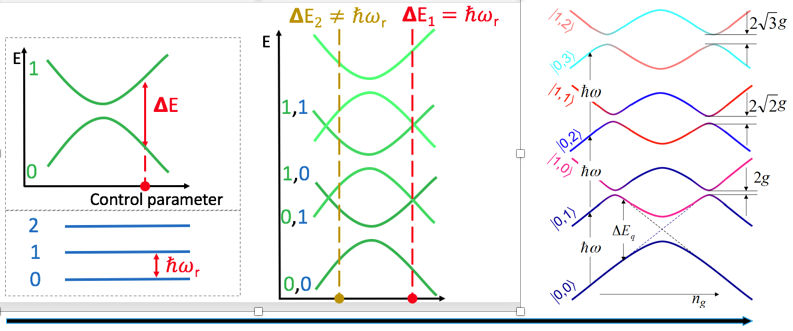
\includegraphics[height=7cm]{d4}
  \caption{We mix  a qubit (with  its typical
    energy  dispersion)   with  a  resonator.
    This  leads to  multiple 'copies'  of the
    qubit   at    the   resonator   frequency
    separations.   These  states  will  cross
    whenever $  \hbar\omega_r\equiv\Delta E $
    i.e.    the   qubit   is  biased   to   a
    configuration   which   is   exactly   in
    resonance  with  the  applied  field  (or
    analogously  we  tune  the  resonator  to
    match the  $ \Delta  E $).   As seen  with the
    above    matrix,   interaction    between
    $\ket{0,N}$ and $ \ket{1,N-1} $ will lift
    the       degeneracy        at       this
    anticrossing.\label{qrDresssed}}
\end{figure}

Now  let  us  perform  measurements  on  this
system.

\begin{itemize}
\item  We  bias  the qubit  to  an  arbitrary
  $ \Delta  E $  and couple  it with  a resonator,
  with frequency $ \omega_r $.
\item Then we send a weak field probe signal,
  measuring its transmission  as we sweep it.
  It  will have  a peak  at the  frequency of
  resonator $  \omega_0 $,  which corresponds
  to the excitation of the qubit.
\item  We plot  the maximum  of this  peak as
  shown in Fig.\ref{qrProbe}.
\item Then we step  the control parameter, to
  move along the qubit curve and repeat.
\item  Everywhere apart  from the  degeneracy
  point, there will be  a single transition -
  the  $   \hbar\omega_0  $  one   that  will
  dominate.
\item However near  the degeneracy point, two
  transitions, symmetrical about $ \omega_0 $
  will be  present.  This is a  result of the
  $ \pm  g_0\sqrt{N} $ splitting  that occurs
  at the crossing point.
\item  Thus  at   the  degeneracy  point  one
  observes two peaks  for the transmission as
  in  Fig.\ref{qrDegen2}  -  the  two  strong
  transitions   at   the   splitting   point.
  Generally the lower peak will be stronger -
  smaller energy difference in the process.
\item The width of the peak $ \gamma $ corresponds
  to the  width of  the level  - the  area to
  which  one   can  excite  to.    One  needs
  $   \gamma<<g_0  $   to   observe  such   a
  transitions.   This  is   fulfilled  for  a
  strong drive.
\end{itemize}

\begin{figure}
  \centering
  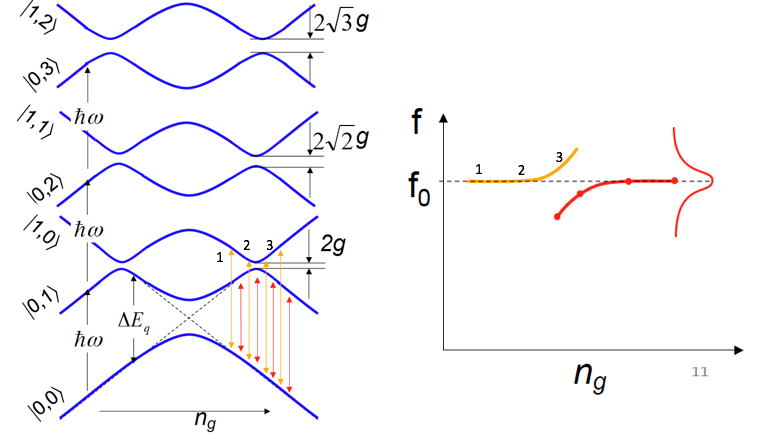
\includegraphics[height=5cm]{probe}
  \caption{We  use  a  weak probe  field  and
    measure its transmission curve.  The peak
    corresponds  to  a favourable  transition
    frequency. \label{qrProbe}}
\end{figure}

\begin{framed}\noindent
  \begin{equation}
    \hbar\Omega_\text{splitting}            =
    2g\sqrt{N},
  \end{equation}

  \noindent   defines   the  Rabi   frequency
  $  \Omega_\text{splitting}  $  and  becomes
  constant for $N>>1$.
\end{framed}

The  configuration  in Fig.\ref{qrDegen2}  is
the Mollow triplet - it is probed either by a
weak field  (as explained above)  or directly
observed in the spectrum emitted by the atom.


\begin{figure}
  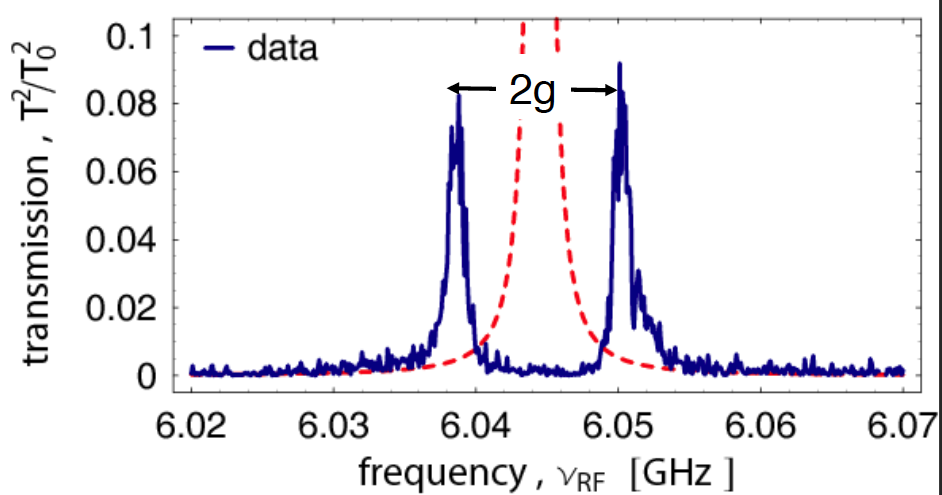
\includegraphics[height=6cm]{degen2}
  \caption{At the degeneracy  point, when the
    resonator field coincides  with the qubit
    transition,  two   types  of  transitions
    appear   from   the  splitting   at   the
    degeneracy    point.     The    splitting
    $ \pm  g_0\sqrt{N} $  will put  two peaks
    either  side of  the  central one  (which
    disappears -  there is no longer  a level
    to    accommodate    this    transition).
    $  \gamma $  characterises  the  width of  the
    split levels  and hence the width  of the
    peak.   If  the  width  is  too  big,  no
    splitting shall be seen.\label{qrDegen2}}
\end{figure}

\begin{figure}
  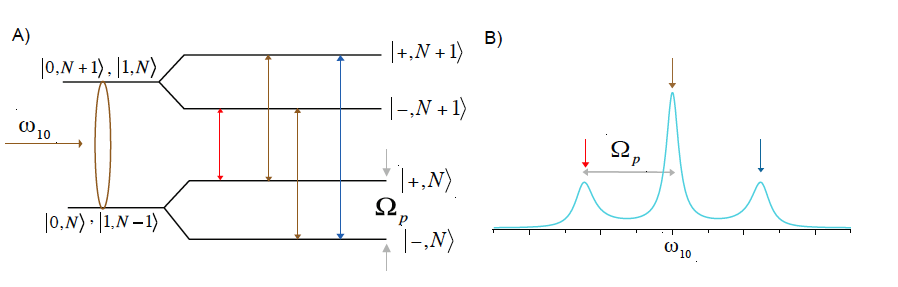
\includegraphics[height=5cm]{tirplet}
  \caption{Mollow  triplet is  formed in  the
    resonant  case.   Three transitions  give
    rise to three peaks.\label{qrMollow}}
\end{figure}

\subsection{Decay rates and quality factors}
\label{sec:decay-rates-quality}

\begin{figure}[h]
  \centering
  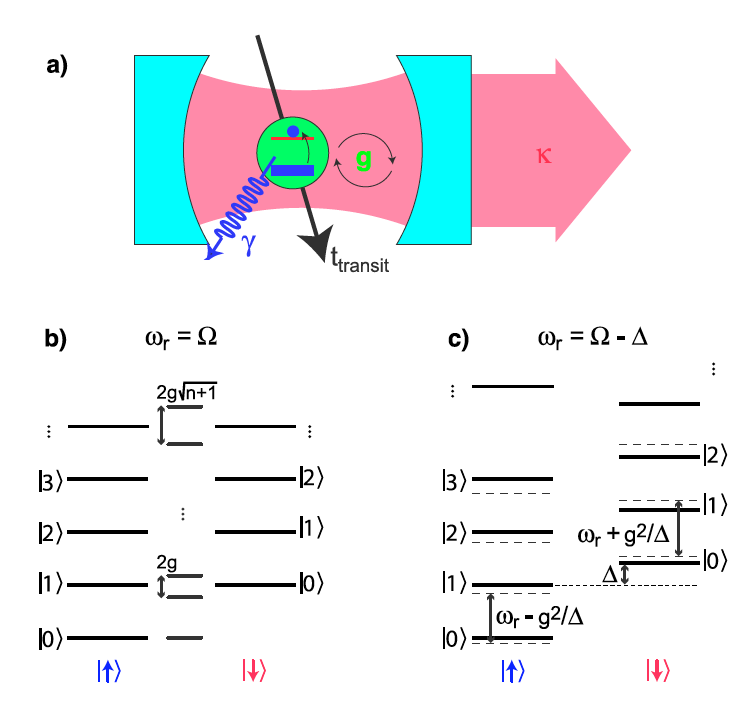
\includegraphics[height=8cm]{cavityPic1}
  \caption{Decay  occurs from  the resonator,
    $\kappa$ or from atom, $\gamma$.}
\end{figure}

There are  two ways  in which the  system can
decay:

\begin{itemize}
\item   Resonator  (cavity)   decay  to   the
  continuum:
  \begin{equation}
    \kappa = \frac{\omega_{r}}{Q}
  \end{equation}

\item  Atom decays  to modes  other than  the
  resonator modes
  \begin{equation}
    \gamma
  \end{equation}
\end{itemize}

\subsection{Second order effects}
Just to  refresh out memory,  our Hamiltonian
has the following form

\begin{equation}\label{sec}
  -\frac{\Delta E}{2}\sigma_x + \hbar\omega_ra^{\dagger}a + \red{\hbar g_0\big(a\sigma^{+}+a^{+}\sigma^{-}\big)},
\end{equation}

\noindent  and  without the  \red{interaction
  term} one had the following eigenstates and
eigenenergies

\begin{equation}\label{secStates}
  \begin{aligned}
    &\ket{n,N}\\
    &\big(n-\frac{1}{2}\big)\Delta E + \hbar\omega
    N.
  \end{aligned}
\end{equation}

\noindent  Now   we  consider   second  order
effects,  where there  is  a frequency  shift
when  the  qubit  is in  the  excited  state.
These  second order  effects will  change the
energies and eigenstates

\begin{equation}\label{secEi}
  E'_{n,N} = E_{n,N}^{(0)} + E_{n,N}^{(1)};\quad \ket{\Psi'_{n,N}}=\ket{\Psi^{(0)}_{n,N}}+\ket{\Psi^{(1)}_{n,N}}+\ket{\Psi^{(2)}_{n,N}}.
\end{equation}


\begin{figure}[h]
  \centering%
  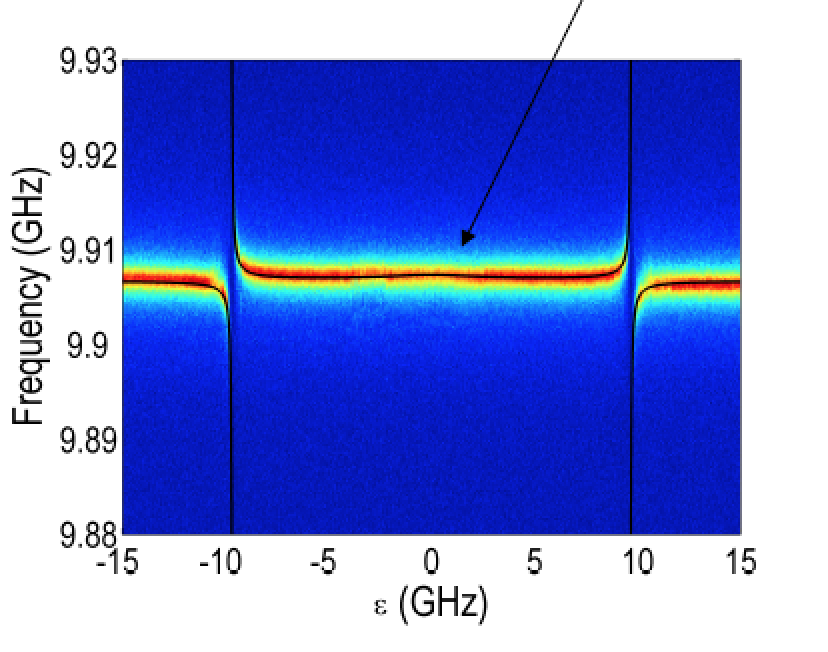
\includegraphics[height=4cm]{shift}
  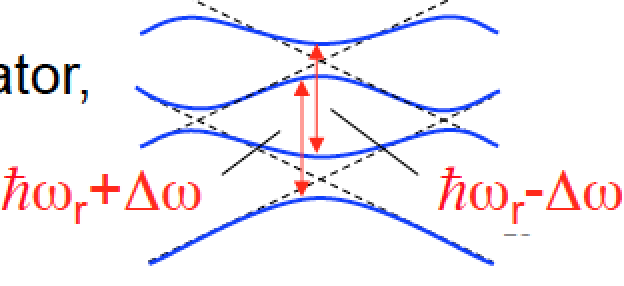
\includegraphics[height=4cm]{sfhit1}
\end{figure}

\noindent From  time independent perturbation
theory, one finds that the first order energy
shift term is

\begin{equation}\label{sec1st}
  E_{n,N}^{(1)} = \bra{\Psi^{(0)}_{n,N}}V\ket{\Psi^{(0)}_{n,N}} = \bra{n,N}g_0\big(a\sigma^{+}+a^{+}\sigma^{-}\big)\ket{n,N} \equiv 0,
\end{equation}

\noindent while the second order energy shift

\begin{equation}\label{sec2nd}
  E_{n,N}^{(2)} = \sum_{m,M}\frac{\left|\bra{m,M}g_0\big(a\sigma^{+}+a^{+}\sigma^{-}\big)\ket{n,N}\right|^2}{E_{n,N}-E_{m,M}}.
\end{equation}

\noindent  For the  two states  of the  qubit
this evaluates to

\begin{equation}\label{sec0}
  E_{0,N}^{(2)} = |g_0|^2\sum_{m,M}\frac{\left|\bra{m,M}\big(a\sigma_{+}+a^{\dagger}\sigma_{-}\big)\ket{0,N}\right|^2}{E_{0,N}-E_{m,M}}= |g_0|^2\frac{\left|\bra{1,N-1}\sqrt{N}\ket{1,N-1}\right|^2}{E_{0,N}-E_{1,N-1}} = -\frac{|g_0|^2N}{\Delta E - \hbar\omega}
\end{equation}

\noindent and

\begin{equation}\label{sec1}
  E_{1,N}^{(2)} = |g_0|^2\sum_{m,M}\frac{\left|\bra{m,M}\big({a\sigma_{+}}+a^{\dagger}\sigma_{-}\big)\ket{1,N}\right|^2}{E_{1,N}-E_{m,M}}= |g_0|^2\frac{\left|\bra{0,N+1}\sqrt{N+1}\ket{0,N+1}\right|^2}{E_{1,N}-E_{1,N-1}} = \frac{|g_0|^2(N+1)}{\Delta E - \hbar\omega \hbar\omega}
\end{equation}

\noindent  From this  we evaluate  the energy
difference   between  atomic   and  resonator
transitions:

\begin{itemize}
\item \textbf{Atomic transition}  can be seen
  to depend  on the number of  photons in the
  resonator

  \begin{equation}\label{secAtom}\begin{aligned}
      E'_{1,N}-E'_{0,N}  & =  E_{1,N}^{(0)} +
      E_{1,N}^{(1)}    +   E_{1,N}^{(2)}    -
      E_{0,N}^{(0)}    -   E_{1,N}^{(1)}    -
      E_{0,N}^{(2)}    \\&    =   \Delta    E    +
      \frac{|g_0|^2(N+1)}{\Delta E  - \hbar\omega}
      -      (-\frac{|g_0|^2N}{\Delta     E      -
        \hbar\omega})\\&         =         {\Delta
        E+\frac{|g_0|^2(2N+1)}{\Delta      E     -
          \hbar\omega}}
    \end{aligned}
  \end{equation}
\item  \textbf{Resonator transition}  depends
  on the state of the qubit

  \begin{equation}\label{secRes}
    E'_{n,N+1}-E'_{n,N} = \left[\begin{aligned}
        & \hbar\omega  -\frac{|g_0|^2}{\Delta E -  \hbar\omega} \text{ for n=0}
        \\&  \hbar\omega + {\frac{|g_0|^2)}{\Delta E -  \hbar\omega}}\text{ for n=1}
      \end{aligned}\right.
  \end{equation}
\end{itemize}

\subsection{Driving qubit-resonator system}
\label{sec:driving-system}

The drive  Hamiltonian for  a qubit-resonator
system  we add  a  coherent  field that  will
couple with the qubit  via the resonator with
the same coupling strength $g$.

\begin{equation}
  \mathcal{H}     =\blue{-\frac{\Delta
      E}{2}\sigma_z}+\blue{{\hbar\omega_r}a^\dagger
    a}             +             \red{\hbar
    g_0\bigg({a\sigma^+}+{a^{\dagger}\sigma^-}\bigg)} + \green{\hbar g \left( \alpha^{*}\sigma^{-}+\alpha\sigma^{+} \right)}.
\end{equation}

\noindent

\subsection{Realisation of resonator}
To realise,  we put  the atom at  the maximum
voltage  of  a   `cut  out'  resonator.  Full
details are given in \cite{Blais_2004}.

\begin{figure}[h]
  \centering
  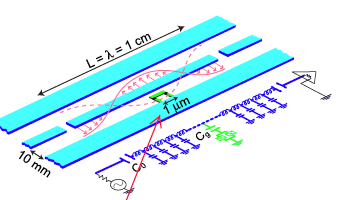
\includegraphics[height=4cm]{cavity_qed_1}
  \caption{Qubit is placed at the antinode of
    resonaotr. The tranmission line itself is
    modelled as a  sequence of capacitors and
    inductors.}
\end{figure}

\noindent
\begin{itemize}
\item  The coupling  strength  is very  large
  because of the small sizes of the elements.
  The  voltage  between theground  plane  and
  resonator  is 0.2\,V/m,which  is 100  times
  stronger than for a regular cavity;
\item The geometry of the resonator fixes its
  frequency \ira no 1/f noise;
\item Atom will emit  directly into the line,
  and  with  a  high enough  quality  factor,
  losses are minimised.
\end{itemize}

\section{Atom - resonator coupling}
\noindent \red{\large \textbf{Solving for the
    Harmonic   oscillator  alone}},   with  a
relaxation rate $ \kappa  $ between the levels, it
is convenient to write  the Linbland term and
the density matrix as

\begin{equation}\label{ar2}
  \mathcal{H} = \hbar\omega_ra^{\dagger}a+\hbar\Omega(a+a^{\dagger})\cos(\omega t);\quad\rho^{(r)} = \sum_{M,N=0}^{\infty}\rho_{NM}^{(r)}\iketbra{N}{M};\quad \mathcal{L}^{(r)} = \frac{\kappa}{2}\bigg(2a\rho a^{\dagger}-a^{\dagger}a\rho-\rho a^{\dagger}a\bigg),
\end{equation}

\noindent  which  ultimately results  in  the
following contribution  to from  the Linbland
term

\begin{equation}\label{ar3}
  \dot{\rho}_{NN}^{(r)} \rightarrow \kappa(N+1)\rho_{N+1\ N+1}^{(r)} - \kappa N \rho_{NN}^{(r)}.
\end{equation}


\begin{enumerate}
\item  The Hamiltonian  for the  resonator is
  transformed    by     moving    into    the
  corresponding rotating frame

  \begin{equation}\label{ar4}
    \mathcal{H'} = -\hbar\delta\omega a^{\dagger}a+\frac{\hbar\Omega}{2}(a+a^{\dagger}).
  \end{equation}

\item  Solving the  Master  equation for  the
  continuous   drive   for   the   stationary
  condition and assuming  that the driving is
  weak  (and  thus  only  the  bottom  photon
  levels will be  occupied), the solution can
  be truncated to have  only the \iket{0} and
  \iket{1} photon states.

  \begin{figure}[h]
    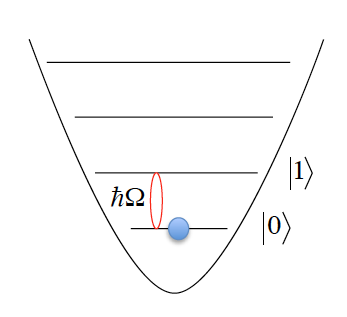
\includegraphics[height=4cm]{resDen1}
    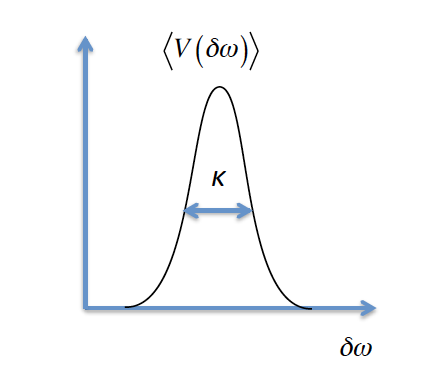
\includegraphics[height=4cm]{resDen2}
  \end{figure}

\item The expectation value  for the field in
  the  resonator is  found using  the density
  matrix for the stationary condition

  \begin{equation}\label{filedRes}
    \iaverage{V} = V_0\iaverage{a+a^{\dagger}} = V_0\itrace{(a+a^{\dagger})\rho}\approx\frac{2\Omega}{\kappa+2\delta\omega},
  \end{equation}

  \noindent which is  a Lorentian, whose peak
  occurs for the case when $ \delta\omega=0 $
  and  the  field  being driven  through  the
  resonator is exactly in resonance with it.
\end{enumerate}

\noindent \red{\large \textbf{Now include the
    atom with the resonator system}}

\begin{equation}\label{ar1}
  \begin{aligned}
    \mathcal{H} & ={-\frac{\Delta E}{2}\sigma_z}+{{\hbar\omega_r}a^\dagger a} + {g_0\bigg({a\sigma^+}+{a^{\dagger}\sigma^-}\bigg)}\\
    &\mathcal{L}^{(a)} = \frac{\Gamma_1}{2}\bigg(2\sigma^{-}\rho \sigma^{+}-\sigma^{+}\sigma^{-}\rho-\rho \sigma^{+}\sigma^{-}\bigg);\quad\mathcal{L}^{(r)} = \frac{\kappa}{2}\bigg(2a\rho a^{\dagger}-a^{\dagger}a\rho-\rho a^{\dagger}a\bigg)\\
    \dot{\rho} & = -\frac{i}{\hbar}\big[\mathcal{H},\rho\big]+\mathcal{L}^{(a)}+\mathcal{L}^{(r)};\quad\quad\quad \rho = \sum_{m,n=0}^{1}\sum_{M,N=0}^{\infty}\rho_{nm,NM}\iketbra{nN}{mM}\\
  \end{aligned}
\end{equation}

\noindent and  this kind  of system  has been
solved  before,  but   now  there  are  decay
mechanisms  also.  The  states  decay with  a
rate

\begin{equation}\label{ardecay}
  \gamma=\frac{\kappa+\Gamma_1}{2},
\end{equation}

\noindent meaning that in order to couple the
qubit and resonator, the energy exchange must
occur  faster  than  this  decay  time.   The
energy    exchange   occurs    at   a    rate
$ \hbar/g_0 << 1/\Gamma_1,1/\kappa$, imposing
the condition that

\begin{equation}\label{arD}
  g_0>>\hbar\Gamma_1,\hbar\kappa,
\end{equation}

\noindent   in  which   the  characteristic7c
energy is higher than incoherent processes.

\begin{figure}[h]
  \centering%
  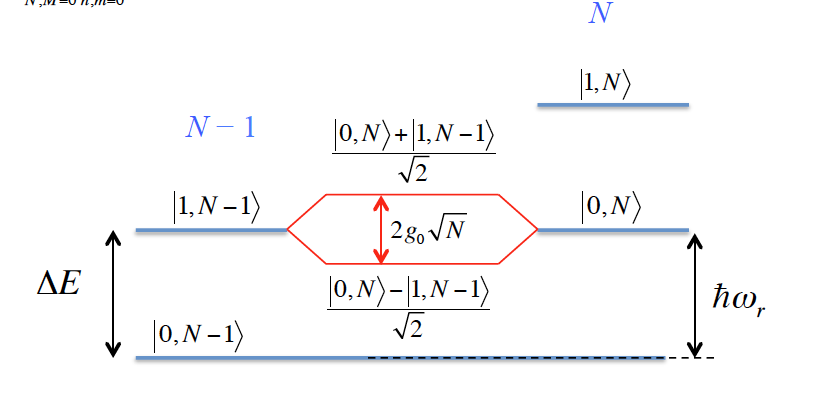
\includegraphics[height=4cm]{ladderGrid}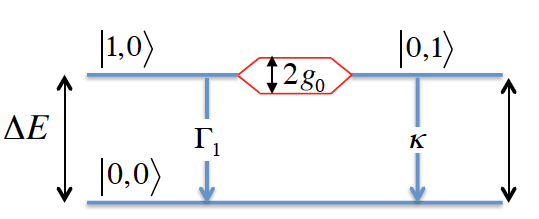
\includegraphics[height=4cm]{ladderGrid1}
  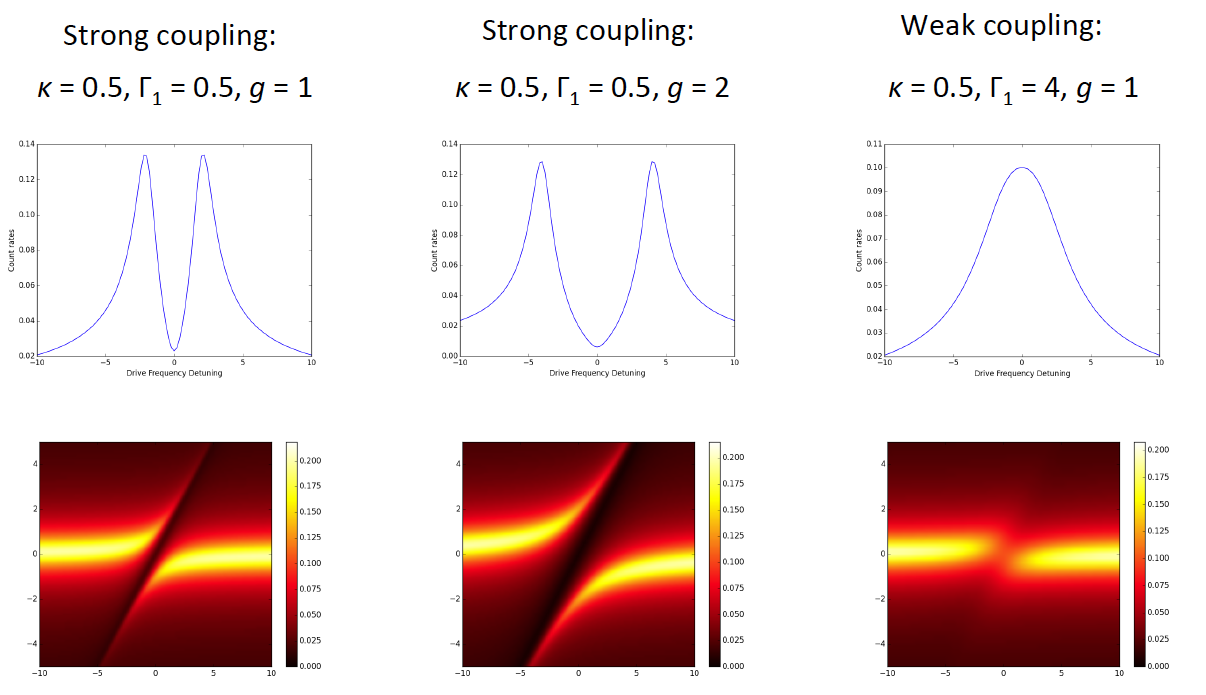
\includegraphics[height=5cm]{coupling}
\end{figure}


\newpage
\section{Measurement with resonator}
\label{sec:meas-with-reson}

There are some simple rules, when it comes to
measuring with a resonator:

\begin{framed}\noindent
  \begin{enumerate}
  \item Current  has nodes on the  end of the
    resonator - voltage has antinodes;
  \item Flux qubit needs current maxima;
  \item Charge qubits need voltage maxima;
  \item  Say the  resonator  has a  resonance
    $  n  =  1  $  of  \iunit{2}{GHz}.   When
    measuring   the   qubit,  each   of   the
    resonance   lines    corresponds   to   a
    particular standing wave profile:
    \begin{center}
      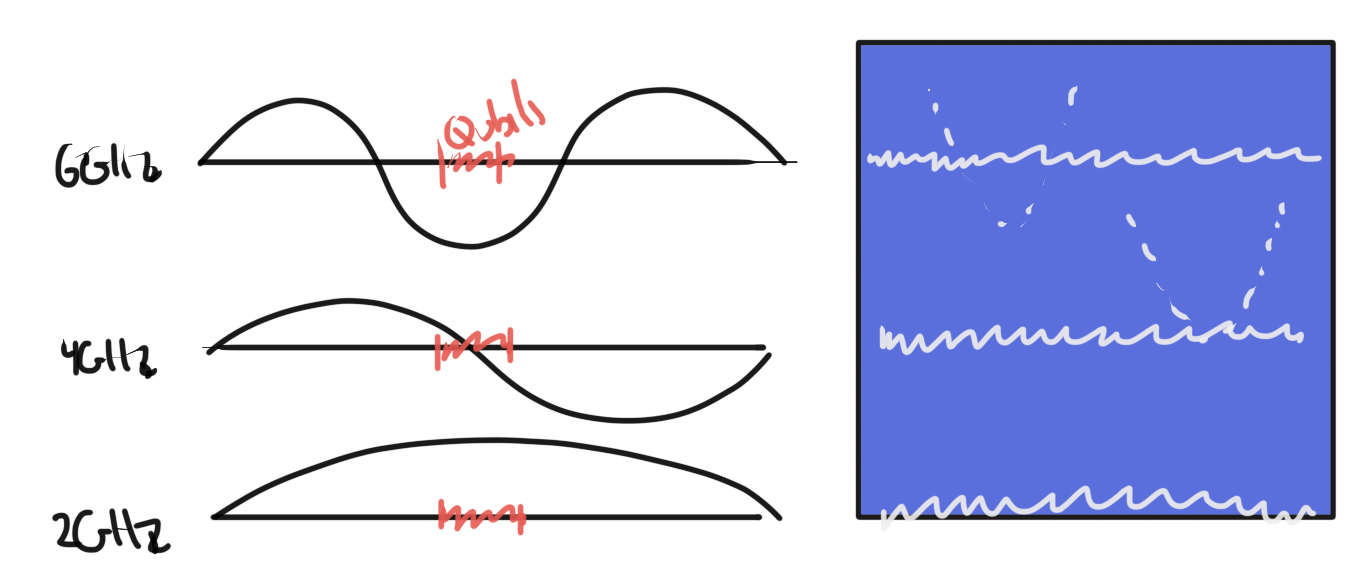
\includegraphics[height=5cm]{qubit_resonator1.png}
    \end{center}
    \noindent  Tune the  VNA  (probe) to  the
    best resonance  for your position  of the
    qubit       in      \red{\textbf{two-tone
        measurements.}}
  \end{enumerate}
\end{framed}

\begin{framed}\noindent
  When making a resonator:
  \begin{enumerate}
  \item The  length of the  resonator effects
    the wavelength $\lambda$  of the standing
    waves;

  \item Speed is determined by
    \begin{equation}
      \label{eq:resonator2}
      v = \frac{1}{\sqrt{LC}}.
    \end{equation}

    \noindent and in turn

    \begin{equation}
      \label{eq:resonator3}
      L      \propto  R \propto  \text{length}/\text{width};
    \end{equation}

  \item Thus, in order to raise the resonator
    frequency \red{\textbf{while  keeping the
        same  standing  wave for  interaction
        with the qubit}},  make the resonator
    \red{\textbf{wider}}.
  \end{enumerate}
\end{framed}

\noindent A useful way  of figuring out which
resonance you are firing with the first tone,
is to look for \textbf{vertical lines} in the
spectrum.     Whenever   the    qubit   cross
\textbf{your  resonance} (e.g.   resonator at
3GHz, and we move to field where the qubit is
at 6GHz) \red{\textbf{then irrelevant of what
    the  generator  sweeps,  the  qubit  will
    always be giving a  response so you get a
    vertical white line.}}

\subsection{Choosing power}
\label{sec:choosing-power}

\begin{enumerate}
\item  For  two-tone measurements,  make  the
  probe signal \red{1st  tone} fairly weak so
  that  there  is  a  single  photon  in  the
  resonator.

  Keep  raising  the power,  until  resonator
  lines become distorted.

\item  The  generator signal  \red{2nd  tone}
  should  be  weak  enough   to  get  a  thin
  response   from  resonator,   but  powerful
  enough to get a response at all.
\end{enumerate}

\newpage
